\documentclass{article}
\usepackage[utf8]{inputenc}

\usepackage{xcolor}

% =============== geometry ===============
\usepackage{geometry}
\geometry{left=2.5cm,right=2.5cm,top=2.5cm,bottom=2.5cm}

% =============== math command ===============
\usepackage{bm}
\usepackage{latexsym,amssymb,amsmath} 
\usepackage{comment}
% flower
\usepackage{mathrsfs}

% =============== graphics ===============
\usepackage{graphicx}

% =============== link color ===============
\usepackage{hyperref}

\newtheorem{theorem}{Theorem}
\newtheorem{lemma}{Lemma}
\newtheorem{definition}{Definition}

\newcommand\numberthis{\addtocounter{equation}{1}\tag{\theequation}}
\newcommand{\oneb}{{\mathbf{1}}}
\newcommand{\lspan}{{\mathrm{span}}}
\newcommand{\Bc}{{\mathcal{B}}}
\newcommand{\Pc}{{\mathcal{P}}}
\newcommand{\Hc}{{\mathcal{H}}}
\newcommand{\Cc}{{\mathcal{C}}}
\newcommand{\Dc}{{\mathcal{D}}}
\newcommand{\Qc}{{\mathcal{Q}}}
\newcommand{\Ic}{{\mathcal{I}}}
\newcommand{\Jc}{{\mathcal{J}}}
\newcommand{\Xc}{{\mathcal{X}}}
\newcommand{\Zc}{{\mathcal{Z}}}

\newcommand{\Lc}{{\mathcal{L}}}
\newcommand{\Nc}{{\mathcal{N}}}

% random vector
\newcommand{\va}{{\mathbf{a}}}
\newcommand{\vx}{{\mathbf{x}}}
\newcommand{\vu}{{\mathbf{u}}}
\newcommand{\vv}{{\mathbf{v}}}
\newcommand{\vh}{{\mathbf{h}}}
\newcommand{\vy}{{\mathbf{y}}}
\newcommand{\vw}{{\mathbf{w}}}
\newcommand{\vW}{{\mathbf{W}}}
\newcommand{\vI}{{\mathbf{I}}}
\newcommand{\vH}{{\mathbf{H}}}
\newcommand{\vtheta}{{\mathbf{\theta}}}
\newcommand{\veps}{{\mathbf{\epsilon}}}

% operator
\newcommand{\inprod}[1]{{\langle{#1}\rangle}}
\newcommand{\CE}[1]{{\text{CE}\{{#1}\}}}
\newcommand{\ddt}[1]{{\frac{d}{dt}{#1}}}
\newcommand{\ppt}[1]{{\frac{\partial }{\partial t}{#1}}}
\newcommand{\inppt}[1]{{\frac{\partial {#1}}{\partial t}}}

%import
\newcommand{\Pb}{{\mathbb{P}}}
\newcommand{\Rb}{{\mathbb{R}}}
\newcommand{\Eb}{{\mathbb{E}}}

%field
\newcommand{\Kf}{{\mathscr{K}}}


\newcommand{\fix}{\marginpar{FIX}}
\newcommand{\new}{\marginpar{NEW}}

\newcommand{\todo}[1]{{\textcolor{red}{[todo: #1]}}}

\newcommand{\yh}[1]{{\textcolor{purple}{[YH: #1]}}}
\newcommand{\diff}[1]{{\textcolor{blue}{#1}}}

\title{SGD Resample}

\begin{document}

%\input{math_command.tex}

\maketitle

\section{Discrete Algorithm}

let $\vx \in \Rb^d$ to denote the input feature and we wish to do regression task, i.e. to approximate respose variable $y=g(x) \in \Rb$ using a three-layer neural network $\hat{y}=f(x)$. The architecture of the neural network is defined as follows:

\begin{equation}
\begin{aligned}
    \vh_1 &= \sigma(\vW^{(1)} \vx) \\
    \vh_2 &= \sigma(\vW^{(2)} \vh_1) \\
    \hat{y} &= \vW^{(3)} \vh_2
\end{aligned}
\end{equation}, where $\vW^{(i)} \in \Rb^{m_i\times m_{i-1}}$ is the weight matrix in $i$-th layer, and $m_i$ is the hidden size in layer $i$, here the input layer is layer $0$ and $m_0 = d$.

The SGD resample algorithm is doing as follows

\begin{itemize}
    \item[1.] minimize empirical loss w.r.t. last layer, the loss function is
    $$\Lc(\vW^{(3)}) = \frac{1}{n}\sum_{i=1}^n (f(x)-y)^2 + \frac{\lambda_3}{1} \|\vW^{(3)}\|_F$$
    \item[2.] resample weights defined in layer 2: minimize the regularization terms w.r.t. weights connected to layer 2 and fix function value in layer 3 invariant:
    $$\Lc(\vW^{(2)}, \vW^{(3)}) = \frac{\gamma}{n}\sum_{i=1}^n (\hat{y}-\hat{y}^{old})^2 + \frac{\lambda_3}{1} \|\vW^{(3)}\|_F + \frac{\lambda_2}{m_2} \|\vW^{(2)}\|_F$$, where $\gamma$ are hyperparameters that control the constraint of invariance of function value, $x^{old}$ denote the respective value $x$ in original neural network.
    \item[3.] resample weights defined in layer 1: minimize the regularization terms w.r.t. weights connected to layer 1 and fix function value in layer 2 invariant:
    $$\Lc(\vW^{(1)}, \vW^{(2)}) = \frac{\gamma}{n}\sum_{i=1}^n \|\vh_2-\vh_2^{old}\|_2^2 + \frac{\lambda_2}{m_2} \|\vW^{(2)}\|_F + \frac{\lambda_1}{m_1} \|\vW^{(1)}\|_F$$.
\end{itemize}

\subsection{Joint Training Results}

The stationary distributions of parameters learned by standard sgd are as follows:

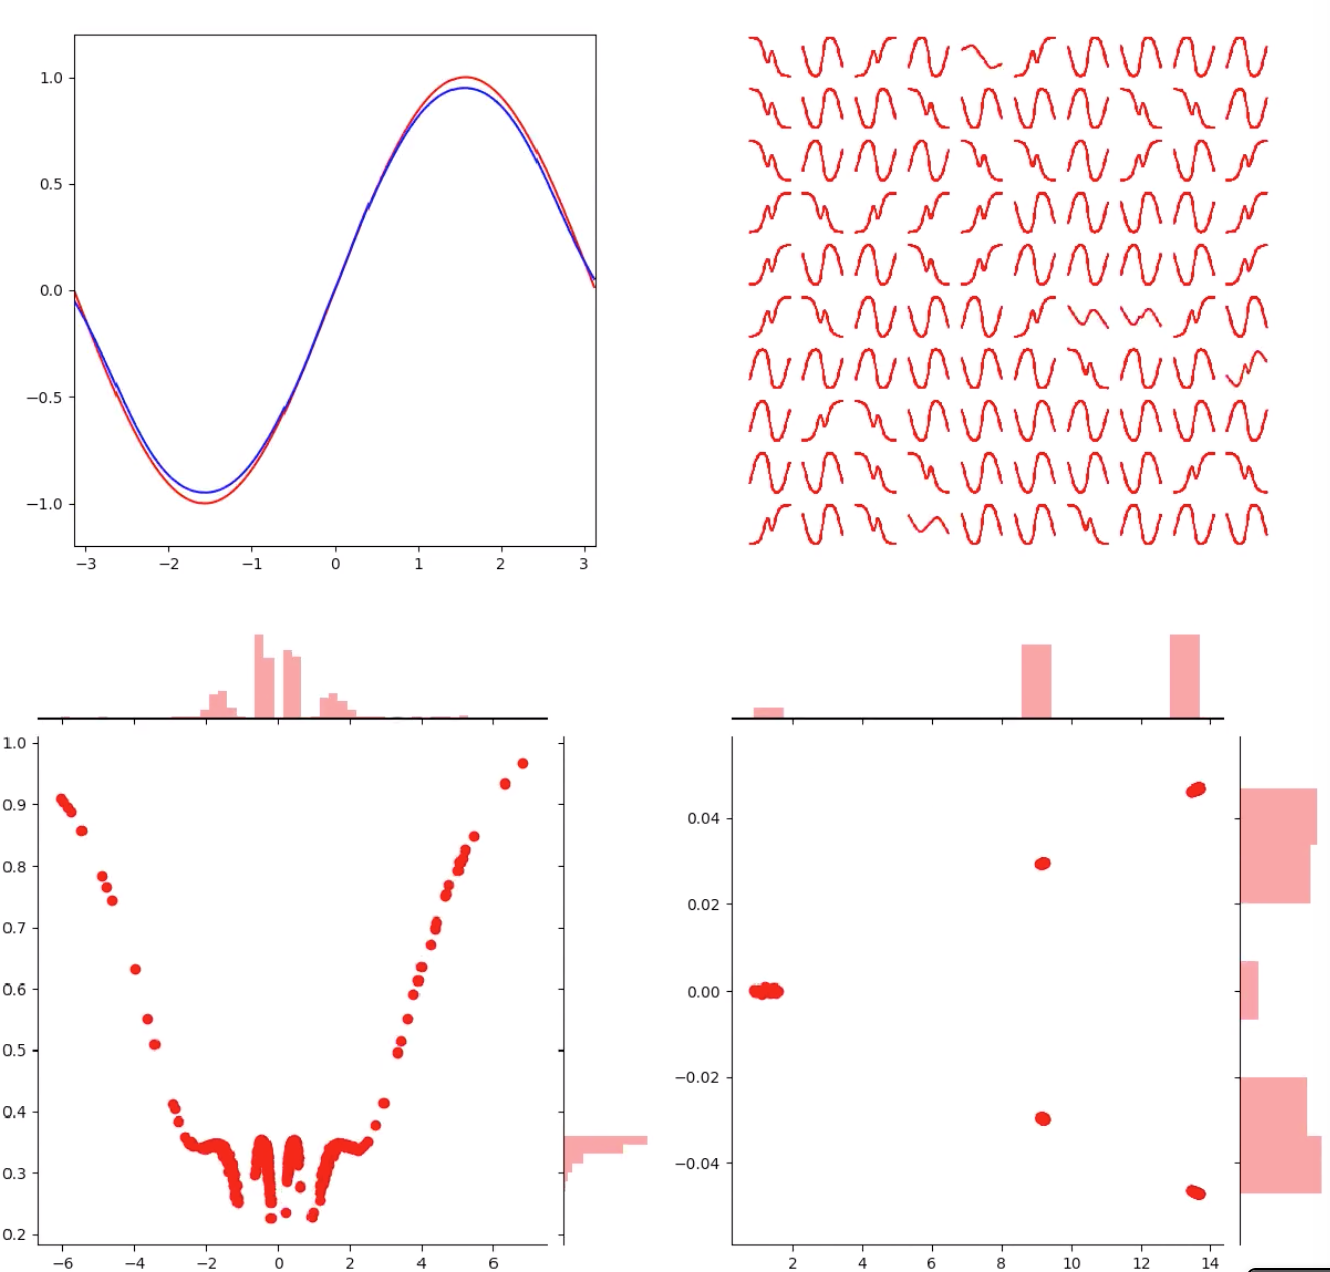
\includegraphics[width=0.7\textwidth]{joint-optimal}

\begin{center}
\begin{tabular}{ |c|c| } 
 \hline
 \emph{prediction function}         & \emph{Samples of $\theta_2$} \\ 
 x: input feature, y: output        & x: input feature, y: response of the neuron $\theta_2$ in layer 2\\ 
 red: groundtruth, blue: prediction & each subplot: a sample of $\theta_2$\\ 
 \hline
 \emph{dist of $\theta_1$ and $\omega(\theta_1)$}                                & \emph{dist of $\|\theta_2\|_2$ and $w(\theta_2)$} \\ 
 x: $\theta_1$, y: $\omega(\theta_1)=\sqrt{\int |\theta_2(\theta_1)|^2 \rho(d\theta_2)}$  & x: $\|\theta_2\|_2$, y: $w(\theta_2)$\\ 
 top and right: marginal histogram                                               & top and right: marginal histogram \\ 
 \hline
\end{tabular}
\end{center}


final regression loss $0.3$e-$3$, regularization loss: $3.0e$-$3$.

\subsection{Steps towards alternative training}

\begin{itemize}
    \item[1.] use well trained $\vW^{(1)}$, and fix them during training: only alternating between step [1] and step [2] in discrete algorithm (video fixedtheta1.mp4)
        \begin{itemize}
            \item final regression loss: $0.3e$-$3$, regularization loss: $2.7e$-$3$
            \item could share similar distribution w.r.t. the conventional sgd algorithm.
            \item attained similar regression loss and smaller regularization loss (and regression loss is more stable)
        \end{itemize}
    \item[2.] use well trained $\vW^{(1)}$ as initialization and alternating between step [1], [2], [3] (video welltheta1.mp4)
        \begin{itemize}
            \item final regression loss: $1.4e$-$3$, regularization loss $2.4e$-$3$.
            \item it seems that the distribution of $\theta_2$ converges quickly but the regression loss converge very slowly.
        \end{itemize}
    \item[3.] use random $\vW^{(1)}$ as initialization, do the original algorithm
        \begin{itemize}
            \item final regression loss: $1e$-$2$
            \item could not converge (both regression loss and distribution)
        \end{itemize}
\end{itemize}

\end{document}

